\chapter{Proposed Methodology}
\label{chap:proposed_methodology}

\section{System Architecture Overview}

The proposed methodology builds upon the GPU-oriented framework described by Martens and Wijs~\cite{martenswijs2024}, which investigates the practical realization of massively parallel algorithms for deterministic finite automaton (DFA) minimization. The framework is designed to evaluate multiple algorithmic paradigms—each derived from well-established theoretical models—and adapt them to exploit the computational capabilities of modern graphics processing units (GPUs). 

The primary objective of this methodology is to reconcile the gap between theoretical parallelism, established in classical works such as Hopcroft~\cite{hopcroft1971} and Paige–Tarjan~\cite{paigetarjan1987}, and real-world GPU execution efficiency. Earlier PRAM-based theoretical models, such as those explored by Tewari et al.~\cite{tewari2002}, established that DFA minimization belongs to Nick’s Class (NC), but did not provide implementable solutions that scale on physical hardware. The present framework seeks to bridge this divide through a unified GPU-based architecture capable of executing and comparing multiple parallel minimization strategies within a controlled experimental setup.

The framework evaluates three algorithmic families:
\begin{enumerate}
    \item \textbf{Transitive Closure-Based Minimization (TRANS)} — A theoretically complete, graph-oriented approach that models equivalence computation as a closure problem.
    \item \textbf{Partition Refinement Algorithms (NaivePR, SortPR)} — Algorithms that iteratively split state partitions based on transition behavior, derived from Hopcroft and Paige–Tarjan’s frameworks.
    \item \textbf{Hybrid Transitive-Partition Minimization (TransPR)} — An adaptive approach combining the transitive closure model with partition refinement to balance iteration depth and per-pass computation.
\end{enumerate}

Each algorithm follows a consistent input–output pipeline, differing primarily in how equivalence between states is computed and refined. By standardizing input formats, GPU kernel configurations, and validation stages, the architecture ensures fair cross-algorithm benchmarking and modular extensibility.

\subsection{Workflow Structure}

The methodology’s overall workflow comprises four major phases, each optimized for concurrent GPU execution:

\begin{itemize}
    \item \textbf{Input and Preprocessing:} The DFA is parsed and transformed into GPU-compatible data structures, using compact, contiguous representations that maximize memory coalescing.
    \item \textbf{Parallel Minimization:} One of the four core minimization algorithms (TRANS, NaivePR, SortPR, or TransPR) is executed using multiple CUDA kernels configured for data-parallel execution.
    \item \textbf{Refinement and Convergence Detection:} Partition updates are performed iteratively until stabilization, with convergence checked using GPU-wide reduction kernels.
    \item \textbf{Output Generation and Validation:} The minimized automaton is reconstructed from the final partition map and cross-verified for equivalence with the original input automaton.
\end{itemize}

This modular decomposition allows different algorithmic strategies to share the same execution environment, ensuring consistent memory handling, data access patterns, and timing metrics. The system design emphasizes minimal kernel-level synchronization and high warp occupancy to achieve near-optimal throughput.

\section{Input Representation and Preprocessing}

The preprocessing stage converts a deterministic finite automaton (DFA) into a flat, GPU-compatible representation. Given a DFA defined as a 5-tuple $(Q, \Sigma, \delta, q_0, F)$, where:
\begin{itemize}
    \item $Q$ is the finite set of states,
    \item $\Sigma$ is the input alphabet,
    \item $\delta: Q \times \Sigma \rightarrow Q$ is the transition function,
    \item $q_0$ is the initial state, and
    \item $F \subseteq Q$ is the set of accepting states,
\end{itemize}
the goal is to encode $\delta$ and $F$ in memory structures conducive to coalesced GPU memory access and efficient thread mapping.

\subsection{Data Transformation}

Traditional CPU representations of DFAs employ pointer-based adjacency lists or transition matrices. However, pointer chasing and irregular access patterns degrade GPU performance. Therefore, all DFA transitions are flattened into contiguous arrays:
\[
\texttt{transitions}[i] = (\texttt{source}_i, \texttt{symbol}_i, \texttt{destination}_i)
\]
This representation guarantees unit-stride memory access and facilitates thread-level parallelism. 

\paragraph{State Encoding:}  
Each DFA state is assigned a unique integer ID in $[0, |Q|-1]$, permitting constant-time indexing of transitions. This enables straightforward mapping between transition entries and partition labels without branching logic.

\paragraph{Transition Compression:}  
Transitions are stored in three parallel arrays (source, symbol, destination), minimizing redundancy. Depending on alphabet size $|\Sigma|$, compressed encoding techniques (e.g., bit-packing for small alphabets) further reduce memory usage.

\paragraph{Initial Partitioning:}  
States are initially grouped into two blocks — accepting and non-accepting — forming the base partition for refinement algorithms. This structure is encoded as a \texttt{partition[]} array storing block identifiers for each state.

\subsection{GPU Memory Preparation}

To ensure efficient execution:
\begin{itemize}
    \item Transitions are aligned to 128-byte boundaries to match GPU cache lines.
    \item Partition and transition arrays are stored in global memory, while block metadata resides in shared memory for frequent updates.
    \item Precomputed offsets and index ranges are maintained for each alphabet symbol to enable symbol-specific kernel launches.
\end{itemize}

This preprocessing step reduces inter-thread memory contention and lays the groundwork for scalable partition updates across thousands of parallel threads.

\section{Core Minimization Algorithms}

The framework implements four core algorithms, each targeting different aspects of DFA equivalence computation. These algorithms share input and output formats but differ in intermediate computation methods and GPU optimization strategies.

\subsection{TRANS — Transitive Closure-Based Minimization}

\textbf{Overview:}  
The TRANS algorithm models DFA minimization as a graph reachability problem. It constructs a \textit{pair graph}, where each node represents a pair of DFA states $(p, q)$. If two states are distinguishable under some input sequence, the pair $(p, q)$ is marked as non-equivalent, and this distinction is propagated through closure computations.

\textbf{Algorithmic Flow:}
\begin{enumerate}
    \item Construct a matrix representing all state pairs $(p, q)$.
    \item Initially mark pairs where one state is accepting and the other is not.
    \item Iteratively propagate distinguishability: if $(\delta(p,a), \delta(q,a))$ is marked, then mark $(p, q)$ as well.
    \item Continue until no new pairs are marked—indicating closure stabilization.
\end{enumerate}

\textbf{Parallelization:}  
On GPUs, each thread is assigned one or more pairs $(p, q)$. Threads evaluate transitions in parallel and perform closure updates using shared bitmaps to represent distinguishability. The propagation phase is implemented as an iterative kernel launch where each pass updates the distinguishability matrix via bitwise OR operations.  

\textbf{Advantages:}
\begin{itemize}
    \item Conceptually simple and mathematically complete.
    \item Highly parallelizable—each pair computation is independent.
\end{itemize}

\textbf{Limitations:}
\begin{itemize}
    \item Quadratic memory complexity $O(|Q|^2)$ restricts scalability.
    \item Iterative closure computation can result in many synchronization rounds.
\end{itemize}

\begin{figure}[H]
  \centering
  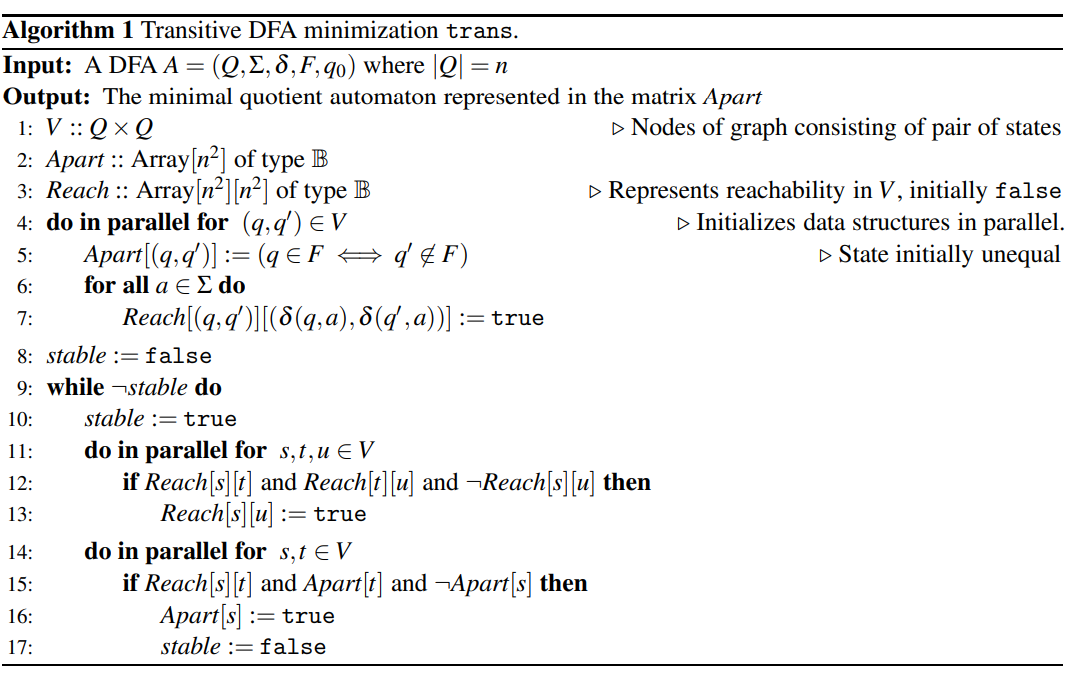
\includegraphics[width=\textwidth,keepaspectratio]{images/trans_1.png}
  \caption{Algorithm 1: Transitive DFA minimization (trans)}
  \label{fig:alg1-trans}
\end{figure}

\subsection{NaivePR — Baseline Partition Refinement Algorithm}

\textbf{Overview:}  
The NaivePR algorithm is a straightforward GPU adaptation of Paige–Tarjan-style refinement. It partitions the state set and repeatedly refines blocks until convergence. This method replaces sequential refinement queues with parallel signature computations, assigning one thread per state.

\textbf{Algorithmic Flow:}
\begin{enumerate}
    \item Initialize two blocks: accepting and non-accepting states.
    \item Compute for each state a \textit{signature}, defined as the vector of destination block IDs for each input symbol.
    \item Sort states by signature; states sharing identical signatures form the same new block.
    \item Repeat until partitions remain unchanged.
\end{enumerate}

\textbf{Leader Selection Variants:}
\begin{itemize}
    \item \textit{Non-atomic (two-phase):} Leaders are elected in a first pass, and new block IDs are assigned in a second.
    \item \textit{Atomic (single-phase):} Compare-and-swap (CAS) atomics are used to claim block leadership immediately.
\end{itemize}

The atomic variant reduces synchronization rounds but may introduce contention under heavy concurrency.

\textbf{Parallel Implementation:}  
Each thread independently computes transition signatures. GPU sorting primitives such as radix sort are employed to group identical signatures efficiently. Reduction kernels detect stable partitions by comparing old and new block IDs.

\textbf{Advantages:}
\begin{itemize}
    \item Minimal control-flow divergence.
    \item Easily extensible to various DFA families.
\end{itemize}

\textbf{Limitations:}
\begin{itemize}
    \item High sorting overhead for large state sets.
    \item Requires multiple refinement iterations to reach stability.
\end{itemize}

\begin{figure}[H]
  \centering
  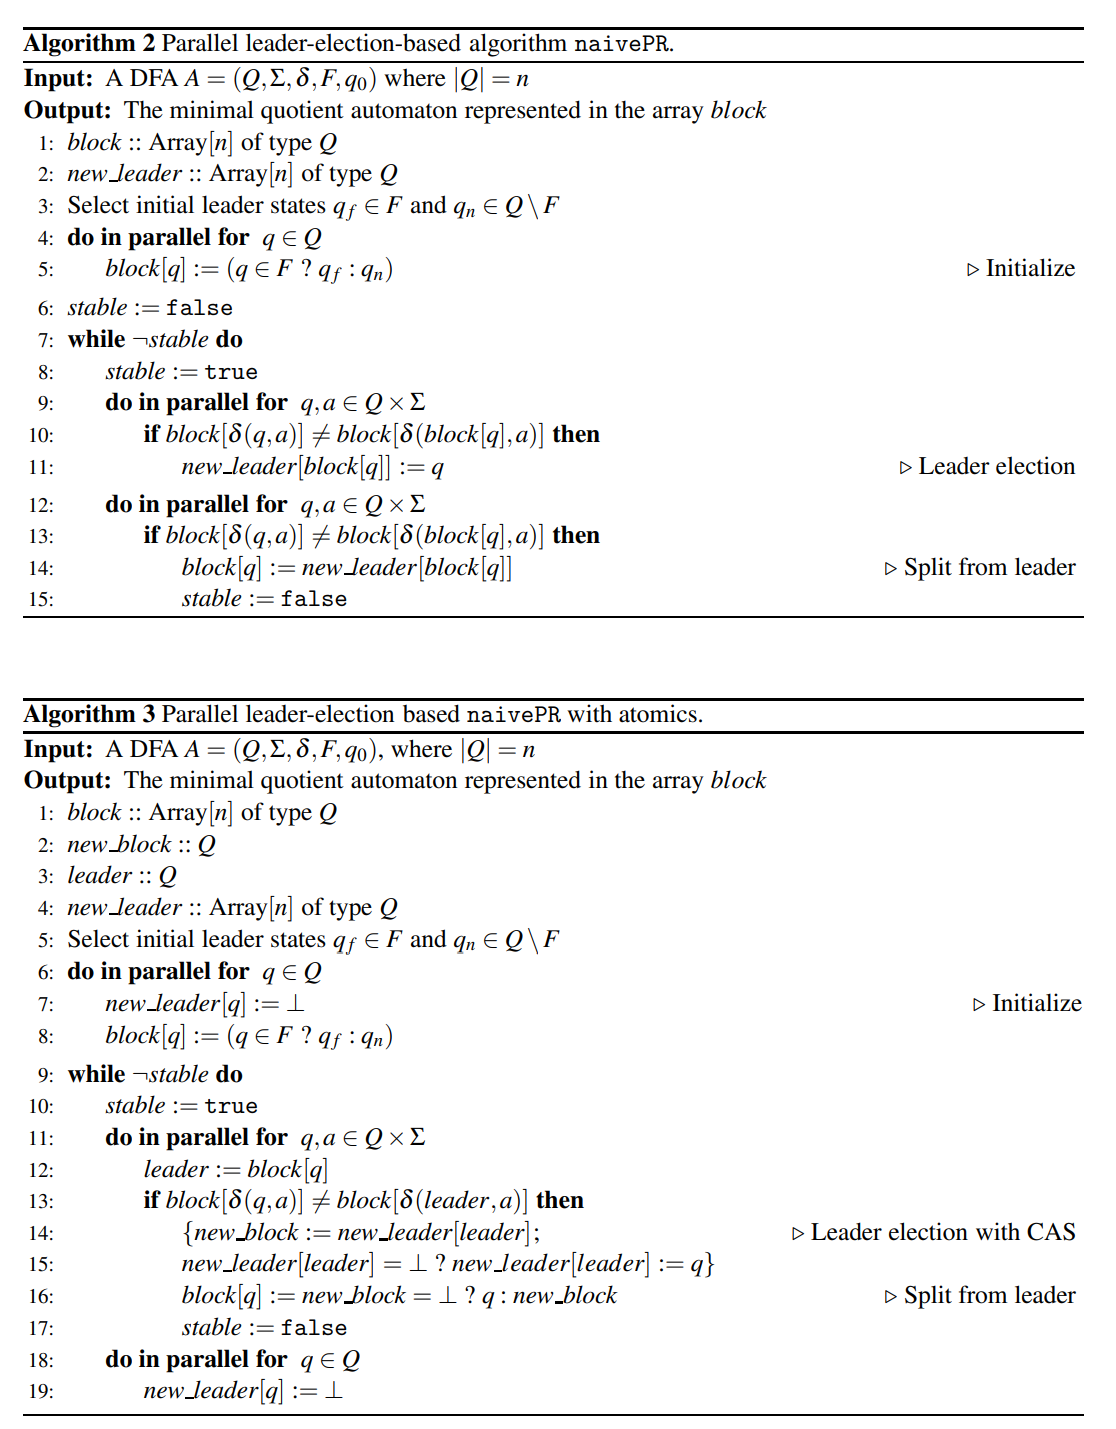
\includegraphics[width=\textwidth,keepaspectratio]{images/naivepr_1.png}
  \caption{Algorithms 2 and 3: NaivePR leader-election variants (non-atomic and atomic)}
  \label{fig:alg2-3-naivepr}
\end{figure}

\subsection{SortPR — Optimized Signature-Based Partition Refinement}

\textbf{Overview:}  
SortPR refines the NaivePR method by employing GPU sorting and hashing optimizations. It minimizes redundant comparisons between states through precomputed signature vectors and hash-based compression.  

\textbf{Algorithmic Flow:}
\begin{enumerate}
    \item Label each transition with its source state and target block ID.
    \item Assemble signature vectors for each state.
    \item Apply parallel radix sort to group identical signatures.
    \item Merge adjacent states with equal signatures into a new block.
    \item Iterate until partitions stabilize.
\end{enumerate}

\textbf{GPU Implementation:}  
SortPR uses shared memory for signature caching and warp-synchronous sorting to minimize divergence. Hash compression ensures signatures fit within per-thread memory limits. Prefix-sum scans efficiently identify block boundaries, eliminating serial bottlenecks.

\textbf{Advantages:}
\begin{itemize}
    \item Outperforms NaivePR by reducing redundant recomputation.
    \item Achieves high GPU occupancy and low synchronization cost.
\end{itemize}

\textbf{Limitations:}
\begin{itemize}
    \item Memory usage increases with large alphabets due to signature vectors.
    \item Sorting dominates runtime for small automata.
\end{itemize}

\begin{figure}[H]
  \centering
  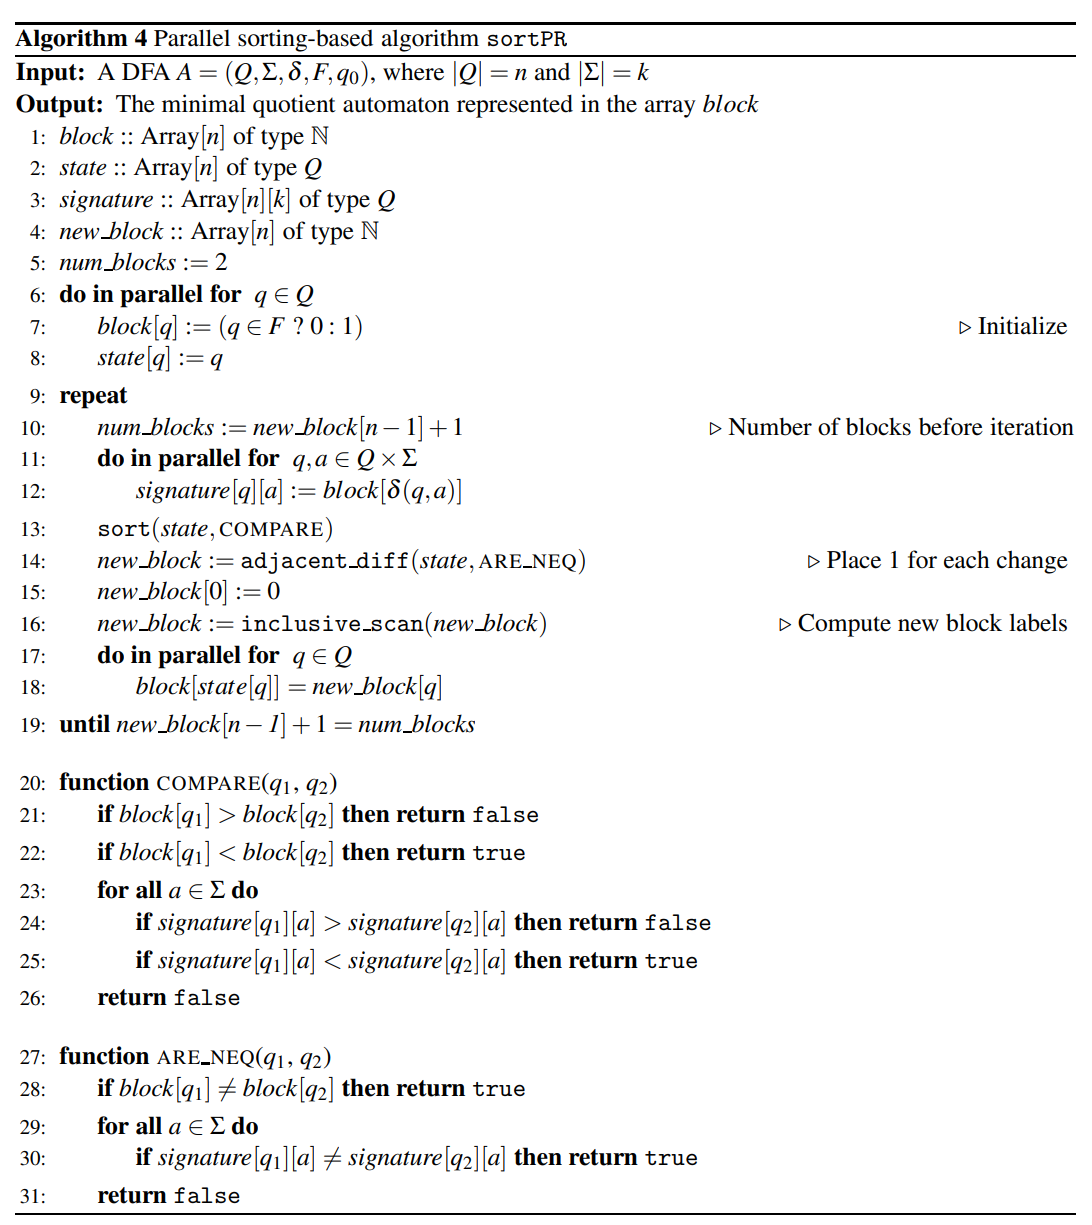
\includegraphics[width=\textwidth,keepaspectratio]{images/sortpr_1.png}
  \caption{Algorithm 4: Parallel sorting-based algorithm (sortPR)}
  \label{fig:alg4-sortpr}
\end{figure}

\subsection{TransPR — Hybrid Transitive-Partition Algorithm}

\textbf{Overview:}  
The TransPR algorithm merges the strengths of both transitive closure and partition refinement approaches. It performs partial closure computations within each iteration to reduce redundant splits, striking a balance between computational depth and per-pass workload.

\textbf{Algorithmic Flow:}
\begin{enumerate}
    \item Begin with partition refinement as in SortPR.
    \item After each iteration, compute closure only on recently modified partitions.
    \item Use closure results to preemptively refine blocks in subsequent iterations.
    \item Alternate between refinement and closure until convergence.
\end{enumerate}

\textbf{Parallel Implementation:}  
The hybrid design launches separate kernels for closure propagation and partition refinement. Shared memory buffers track “changed” partitions, while global synchronization occurs only between kernel phases. This design minimizes global atomic operations.

\textbf{Advantages:}
\begin{itemize}
    \item Reduces total iterations significantly compared to NaivePR.
    \item Balances computational load across threads dynamically.
    \item Demonstrates high performance consistency across diverse automata.
\end{itemize}

\textbf{Limitations:}
\begin{itemize}
    \item More complex to implement due to interleaving phases.
    \item Requires parameter tuning for closure frequency.
\end{itemize}

\begin{figure}[H]
  \centering
  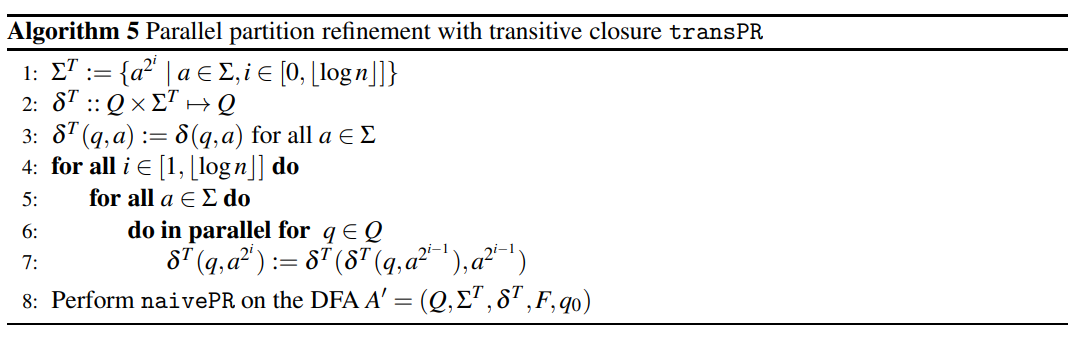
\includegraphics[width=\textwidth,keepaspectratio]{images/transpr_1.png}
  \caption{Algorithm 5: Parallel partition refinement with transitive closure (transPR)}
  \label{fig:alg5-transpr}
\end{figure}

\section{GPU Optimization and Parallel Design Principles}

High performance in GPU computation arises not only from algorithmic parallelism but also from architectural alignment. The following design principles underlie all implementations in this framework:

\begin{itemize}
    \item \textbf{Memory Coalescing:} Data structures are arranged contiguously, enabling adjacent threads to access consecutive memory addresses.
    \item \textbf{Shared Memory Utilization:} Frequently accessed data—such as block metadata—is cached in low-latency shared memory, reducing global access frequency.
    \item \textbf{Warp-Level Synchronization:} Each warp processes sequential blocks of states to minimize divergence and branch mispredictions.
    \item \textbf{Atomic-Free Reductions:} Aggregation operations (such as block splitting detection) employ prefix-sum and reduction primitives instead of atomic counters.
    \item \textbf{Double Buffering:} Alternating input/output buffers prevent race conditions between successive iterations.
\end{itemize}

Additionally, GPU-specific optimizations like register reuse, memory alignment, and warp shuffles are applied to sustain high throughput across millions of concurrent threads.

\section{Implementation Workflow Summary}

All four algorithms are integrated into a common GPU software stack, ensuring modularity and comparability.

\textbf{DFA Loading and Normalization:}
\begin{itemize}
    \item Input automata are parsed into standardized data structures compatible with GPU kernels.
    \item States are labeled, and transition tables are flattened into contiguous arrays.
\end{itemize}

\textbf{Parallel Minimization Stage:}
\begin{itemize}
    \item One algorithm (TRANS, NaivePR, SortPR, or TransPR) is selected at runtime.
    \item Kernels are launched iteratively until convergence.
\end{itemize}

\textbf{Minimized DFA Reconstruction:}
\begin{itemize}
    \item The final partition array is used to construct the minimized DFA.
    \item Transition tables are compacted and exported for analysis.
\end{itemize}

\textbf{Output Validation:}
\begin{itemize}
    \item Behavioral equivalence between the minimized and original DFA is verified using GPU-accelerated equivalence checking.
\end{itemize}

This pipeline allows controlled experimentation, scalability testing, and future integration of additional minimization algorithms.

